\documentclass{beamer}
%\documentclass[handout]{beamer}

% language settings
%\usepackage{fontspec, polyglossia}
%\setdefaultlanguage{magyar}

% common packages
\usepackage{amsmath, multimedia, hyperref, color, multirow}
%\usepackage{graphicx}

% TikZ
\usepackage{tikz}
%\usetikzlibrary{arrows.meta, decorations.pathmorphing, decorations.pathreplacing, shapes.geometric,mindmap}
%\usetikzlibrary{shapes.geometric,fadings,bayesnet}

% beamer styles
\mode<presentation>{
\usetheme{Warsaw}
%\usetheme{Antibes}
\usecolortheme{beaver}
%\usecolortheme{seahorse}
%\usefonttheme{structureitalicserif}
\setbeamercovered{transparent}
}
\setbeamertemplate{blocks}[rounded][shadow=true]
\AtBeginSubsection[]{
  \begin{frame}<beamer>{Contents}
    \tableofcontents[currentsection,currentsubsection]
  \end{frame}
}
%\useoutertheme[]{tree}

% title, etc
\title{Somatic Mutations in the Human Brain from NGS data}
%\subtitle{A subtitle may be shorter and more technical}
\author{Attila Gulyas-Kovacs}
\date{Chess Lab}

\begin{document}

\maketitle

\begin{frame}{Genetics of psychiatric disorders}
\begin{itemize}
\item germline variants
\item \textit{de novo} variants
\item<2-> gene-gene and gene-environment interactions  
\item<3-> somatic variants
\begin{itemize}
%\item<3-> \alert{our hypothesis: psychiatric disorders; schizophrenia}
\item cancer, aging
\item V(D)J recombination
\item dysplasias: hemimegencephaly, lissencephaly, pediatric epilepsy 
\item<4-> \alert{psychiatric disorders?}\\
Brain Somatic Mosaicism Network (BSMN)
\end{itemize}
\end{itemize}
\end{frame}

\begin{frame}{Patterns of somatic mosaicism}
\includegraphics[width=1.0\textwidth]{figures/from-others/lodato2015science-fig3ab.png}
\end{frame}

\begin{frame}{Embryonic development}
%gastrulation video
%https://www.youtube.com/watch?v=3AOoikTEfeo
%neurulation video
%https://www.youtube.com/watch?v=lGLexQR9xGs
\includegraphics[height=0.8\textheight]{figures/from-others/HumanEmbryogenesis.png}
\end{frame}

\begin{frame}{Neocortical development}
\includegraphics[height=0.8\textheight]{figures/from-others/doi_10_1016-j_cell_2011_06_030-fig4b-neocortical-development.jpg}
\end{frame}

\begin{frame}{Mutation rate}
\includegraphics[width=0.8\columnwidth]{figures/from-others/lynch-evolution-of-mutation-rate-fig3.jpg}
\end{frame}

\begin{frame}{Sequencing approaches to detect somatic variants}
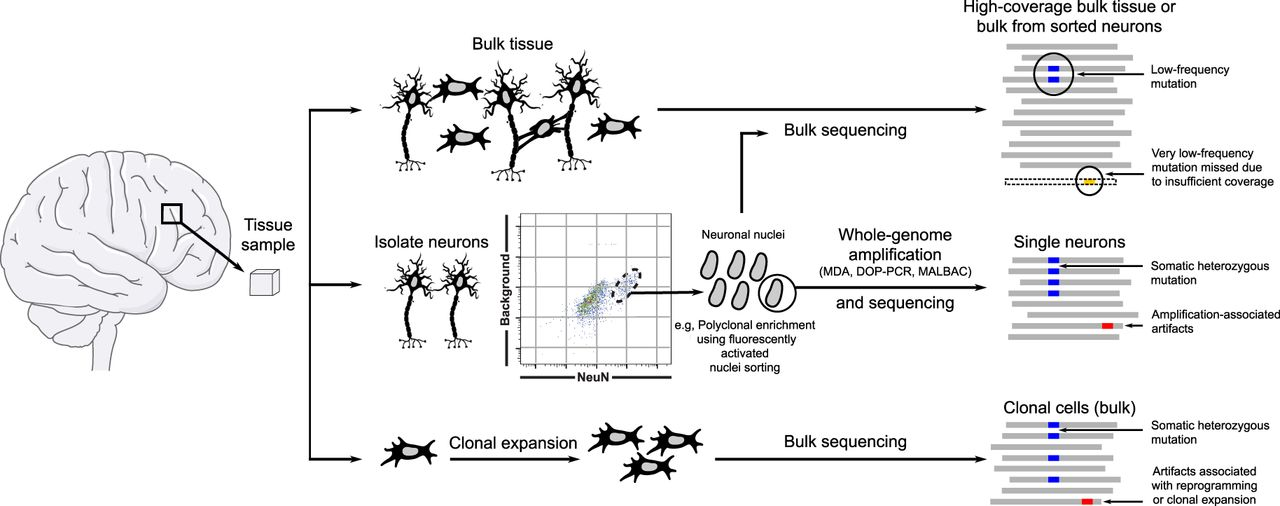
\includegraphics[width=1.0\textwidth]{figures/from-others/bsm-science-fig2.jpg}
\end{frame}

\end{document}


\begin{columns}[t]
\begin{column}{0.5\textwidth}

\end{column}

\begin{column}{0.5\textwidth}

\end{column}
\end{columns}
